    
\documentclass[]{scrreprt}
\usepackage{listings}
\usepackage{graphicx}
\lstset{numbers=left}
%opening
\title{Systemsicherheit - 2. Übung}
\author{Dennis Rotärmel, Niklas Entschladen, Tobias Ratajczyk, Gruppe Q}

\begin{document}
	
	\maketitle
	\chapter{Aufgabe 1}
	\subsection*{a)}
	Folgender Assembly-Code führt die Berechnung aus:
	\begin{lstlisting}[caption={Assembler Code "Erstes Programm"},captionpos=b]
	imul ecx, ecx ;ecx*ecx
	sub ecx, ebx ;ecx*ecx-ebx
	shl eax, 1 ;eax*2
	add eax, ecx ;ecx*ecx-ebx+eax*2
	add ebx, 0xaaaa ;ebx+0xaaaa
	xor eax, ebx ;(ecx*ecx-ebx+eax*2)^(ebx+0xaaaa)
	\end{lstlisting}
	Die Ausgabe des Programms lautet: \texttt{12345}.
	\subsection*{b)}
	Folgender Assembly-Code führt den Primzahltest aus, wobei die Teilbarkeit durch die Zahlen von 2 bis 31 geprüft wird:
	\begin{lstlisting}[caption={Assembler Code "Primzahltest"},captionpos=b]
	; ---- DO NOT MODIFY THE DATA SECTION ----
	section .data
	
	string_choice: db "Choose a number: ", 0
	string_success: db "%d is prime.", 0xa, 0
	string_failure: db "%d is not prime.", 0xa, 0
	string_error: db "Invalid input. Exiting...", 0xa, 0
	input_number: db "%d", 0
	
	; ---- DO NOT MODIFY THE BSS SECTION ----
	section .bss
	choice: resd 1
	
	section .text
	
	global main
	;; tell NASM that printf and scanf are symbols
	;; defined in another module
	extern scanf, printf
	
	; ---- Your code goes into the TODO snippets ----
	
	main:
	;-------------------------------
	; TODO
	; Ask user for input of a number (use string_choice)
	push string_choice
	call printf
	add esp, 4
	;-------------------------------
	
	;-------------------------------
	; TODO
	; Read user input (use input_number)
	push choice ;Trage uebergegebenen Wert in "choice" ein
	push input_number
	call scanf
	add esp, 8
	;-------------------------------
	
	;-------------------------------
	; TODO
	; Check if user input is within valid range
	mov eax, [choice]	; Bewege "choice" in EAX
	cmp eax, 2			; Fehlermeldung, falls choise<2
	jb error
	cmp eax, 1000		; Fehlermeldung, falls choise>1000
	ja error
	mov esi, [choice]
	;-------------------------------
	
	;-------------------------------
	; DO NOT MODIFY THIS
	; Call is_prime subroutine
	mov eax, [choice]  ; Load user input
	push eax           ; Pass user's input via the stack
	call is_prime      ; Call subroutine
	add esp, 4         ; Cleanup stack
	
	; Check result (which is in eax)
	cmp eax, 1
	je success
	
	; If number is not prime, print failure message
	push esi
	push string_failure
	call printf
	add esp, 8
	ret 
	
	; If number is prime, print success message
	success:
	push esi
	push string_success
	call printf
	add esp, 8
	ret
	;-------------------------------
	
	;-------------------------------
	; TODO
	; Print error message (use string_error)
	error:
	push string_error
	call printf
	add esp, 4
	ret
	;-------------------------------
	
	;-------------------------------
	; TODO
	; The function is_prime should contain your primality test.
	; Return 1 if the argument (passed via the stack) is prime, else 0.
	; Mark instructions belonging to the prologue and epilogue.
	set_eax_true:
	mov eax, 1
	leave
	retn
	set_eax_false:
	mov eax, 0
	leave
	retn
	is_prime:
	; prologue
	push ebp
	mov ebp, esp
	sub esp, 4h
	; end of prologue
	
	; function body
	mov eax, [ebp+8]
	xor edx, edx
	mov ebx, 2
	cmp eax, ebx		;falls die Eingabe = dem Teiler entspricht
	je set_eax_true
	div ebx
	cmp edx, 0
	jz set_eax_false
	mov eax, [ebp+8]
	xor edx, edx
	mov ebx, 3
	cmp eax, ebx
	je set_eax_true
	div ebx
	cmp edx, 0
	jz set_eax_false
	mov eax, [ebp+8]
	xor edx, edx
	mov ebx, 5
	cmp eax, ebx
	je set_eax_true
	div ebx
	cmp edx, 0
	jz set_eax_false
	mov eax, [ebp+8]
	xor edx, edx
	mov ebx, 7
	cmp eax, ebx
	je set_eax_true
	div ebx
	cmp edx, 0
	jz set_eax_false
	mov eax, [ebp+8]
	xor edx, edx
	mov ebx, 11
	cmp eax, ebx
	je set_eax_true
	div ebx
	cmp edx, 0
	jz set_eax_false
	mov eax, [ebp+8]
	xor edx, edx
	mov ebx, 13
	cmp eax, ebx
	je set_eax_true
	div ebx
	cmp edx, 0
	jz set_eax_false
	mov eax, [ebp+8]
	xor edx, edx
	mov ebx, 17
	cmp eax, ebx
	je set_eax_true
	div ebx
	cmp edx, 0
	jz set_eax_false
	mov eax, [ebp+8]
	xor edx, edx
	mov ebx, 19
	cmp eax, ebx
	je set_eax_true
	div ebx
	cmp edx, 0
	jz set_eax_false
	mov eax, [ebp+8]
	xor edx, edx
	mov ebx, 23
	cmp eax, ebx
	je set_eax_true
	div ebx
	cmp edx, 0
	jz set_eax_false
	mov eax, [ebp+8]
	xor edx, edx
	mov ebx, 29
	cmp eax, ebx
	je set_eax_true
	div ebx
	cmp edx, 0
	jz set_eax_false
	mov eax, [ebp+8]
	xor edx, edx
	mov ebx, 31
	cmp eax, ebx
	je set_eax_true
	div ebx
	cmp edx, 0
	jz set_eax_false
	call set_eax_true
	; end of function body
	
	; epilogue
	leave
	retn
	; end of epilogue / end of function
	;-------------------------------
	\end{lstlisting}
	\chapter{Aufgabe 2}
	\subsection*{a)}
	Bei der Ausführung des Programmes wird der jeweils i-te Buchstabe um den Wert i-1 erhöht (siehe ASCII-Tabelle).
	Danach wird der daraus entstehende String mit folgendem String vergleichen: "HPFRV".
	Daraus lässt sich schlussfolgern, dass das Schlüsselwort "HODOR" lautet. Die Eingabe des Wortes bestätigt dies.
	Bis auf den Befehl "break verif\_key" und die dazugehörigen step- und continue-Anweisungen wurden keine weiteren Befehle benötigt.
	\subsection*{b)}
	\begin{lstlisting}[caption={Crackme-Code},captionpos=b]
	#include <stdio.h>
	
	int verify_key(char *str){
	char key[5] = "HPFRV";
	
	for(int i=0; i<5; i++){
	if (str[i]!=key[i]){
	printf("Key is not valid :(\n");
	return 0;
	}
	}
	printf("Key is valid! Whoop whoop :)\n");
	return 0;
	}
	
	int main(){
	char str[5];
	printf("Enter serial (5 capital letters): ");
	scanf("%s", str);
	
	for(int i=0; i<5; i++){
	str[i]=str[i]+i;
	}
	
	return verify_key(str);
	}
	\end{lstlisting}
	\chapter{Aufgabe 3}
	\subsection*{a)}
	\begin{itemize}
		%\begin{itemize}
		\item \textbf{Data Movement}:
		\item \texttt{mov esi, 4} $\rightarrow$ Speichert den Wert 4 im esi-Register
		\item \texttt{push 2} $\rightarrow$ Bewegt den Wert 2 auf den Stack
		\item \texttt{push esi} $\rightarrow$ Bewegt den Wert des esi-Registers (4) auf den Stack
		\item \texttt{mov eax, dword ptr [esp]} $\rightarrow$ Der Wert, auf den der esp zeigt (4), wird in das eax-Register geladen $\rightarrow$ eax = 4
		\item \texttt{lea eax, [esp + eax * 2 + 4]} $\rightarrow$ Die Adresse des esp, addiert mit dem doppelten Wert des eax und der Konstanten 4, wird in das eax-Register geladen $\rightarrow$ eax = esp+12
		\item \texttt{sub eax, 8} $\rightarrow$ Vom eax-register wird der Wert 8 abgezogen $\rightarrow$ eax = esp+4
		\item \texttt{mov eax, dword ptr [eax]} $\rightarrow$ In das eax wird der Wert an der Stelle [esp+4] geladen $\rightarrow$ eax = 2
		\item \texttt{pop ebx} $\rightarrow$ Der ursprüngliche Wert des esi-Registers wird in das ebx-Register geschrieben und vom Stack entfernt $\rightarrow$ ebx = 4
		\item \texttt{add esp, 4} $\rightarrow$ Der esp wird 4 Bytes nach oben verschoben (bezüglich des Stacks) $\rightarrow$ Der Stack wird aufgeräumt
		\item \texttt{add eax, ebx} $\rightarrow$ eax = 2 + 4 = 6
		%\end{itemize}
		\item  \textbf{Arithmetic and Logic}:
		\begin{itemize}
			\item \texttt{xor eax, eax} $\hat{=}$ eax $\oplus$ eax = 0
			\item \texttt{add eax, 1234h} $\hat{=}$ eax + 4660 = 0 + 4660 = 4660
			\item \texttt{ror eax, 16} $\hat{=}$ {0001001000110100}\textsubscript{2} $\rightarrow$ {0011010000010010}\textsubscript{2} $\hat{=}$  {13330}\textsubscript{10}
			\item \texttt{or eax, 55h} $\hat{=}$ {0011010000010010}\textsubscript{2} $\vee$ {0000000001010101}\textsubscript{2} = {0011010001010111}\textsubscript{2} $\hat{=}$ {13399}\textsubscript{10}
			\item \texttt{inc eax} $\hat{=}$ = eax + 1 = 13400
			\item \texttt{shl ax, 8} $\hat{=}$ 0011010001011000\textsubscript{2} $\rightarrow$ 0011010001011000\textsubscript{2} (ax = 0, somit keine Änderung)
			\item  \texttt{mov al, 78h} $\hat{=}$ 0011010001011000\textsubscript{2} $\rightarrow$ 0011010001110100\textsubscript{2} $\hat{=}$ 13428\textsubscript{10}
			\item Damit ist am Ende der Wert 13428 im \texttt{eax} Register
		\end{itemize}
		
		\item \textbf{Control Flow}:
		\begin{itemize}
			\item \texttt{mov eax, 1h} $\hat{=}$ eax = 00\dots0001
			\item \texttt{neg eax} $\hat{=}$ eax = 11\dots1111
			\item \texttt{mov ebx, FFFFFFF8h}
			\item \texttt{cmp eax, ebx} 
			\item \texttt{jg true} $\rightarrow$ ebx ist größer als eax (da Vorzeichen beachtet)
			\item \texttt{mov eax, 0} wird ausgeführt
			\item damit ist im eax der Wert 0 am Ende.
		\end{itemize}
	\end{itemize}
	\subsection*{b)}
	\texttt{ja} ist ein unsigned-Vergleich, damit wird beim vergleichen das Vorzeichen nicht beachtet. In diesem Fall ist der Wert im \texttt{eax} größer und es wird \texttt{mov eax, 1} ausgeführt.
	\chapter{Aufgabe 4}
	\subsection*{a)}
	\begin{lstlisting}[caption={Funktionen f und g},captionpos=b]
	int fkt_f(int a, int b, int c){
	int d = 0;
	if(a!=0){
	d = fkt_g(a,b);
	}
	else{
	d = a+b;
	}
	int e = c+d;
	return e;
	}
	int fkt_g(int a, intb){
	int f = 0;
	if(f<b){
	a = a+b;
	f = 1;
	}
	return a;
	}
	\end{lstlisting}
	\subsection*{b)}
	Calling Convention: cdecl\\
	Der Caller ruft erst die Subroutine auf (call $\dots$) und gibt danach in der nächsten Instruktion wieder den Platz im Stack frei (add esp, $\dots$). Außerdem werden sämtliche Paramter über den Stack übergeben.
	\begin{itemize}
		\item 1. Paramter: \texttt{[ebp+8]}
		\item 2. Paramter: \texttt{[ebp+0Ch]}
		\item 3. Paramter: \texttt{[ebp+10h]}
	\end{itemize}
\begin{figure}[h]
	\centering
	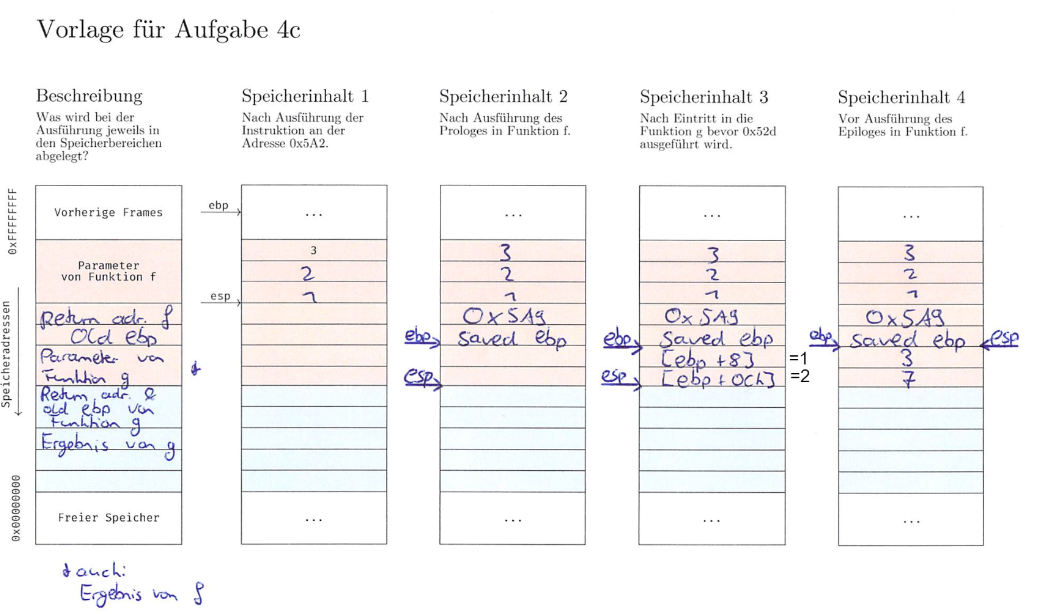
\includegraphics[width=1.2\textwidth]{figure/4b.png}
	\caption{Zustände des Stacks}
\end{figure}
\end{document}